\apendice{Documentación de usuario}

\section{Introducción}
Esta sección tiene como objetivo proporcionar a los usuarios las instrucciones necesarias para instalar, configurar y utilizar la aplicación Eco City Tours. Este manual está dirigido a usuarios finales interesados en explorar ciudades de manera sostenible, sin necesidad de conocimientos técnicos avanzados.
En primer lugar, se describirán los requisitos mínimos necesarios para ejecutar la aplicación. A continuación, se detallarán los pasos necesarios para instalarla. Finalmente, se presentará una guía práctica para que el usuario pueda aprovechar todas las funcionalidades que ofrece la aplicación.
\section{Requisitos de usuarios}
Para garantizar el correcto funcionamiento de \textbf{Eco City Tours}, el dispositivo debe cumplir con los siguientes requisitos:

\subsection*{Requisitos del Sistema Operativo}
\begin{itemize}
	\item \textbf{Versión mínima de Android:} 6.0 (API 23, Marshmallow).
	\item \textbf{Versión objetivo de Android:} 14 (API 34, Upside Down Cake).
	\item La aplicación está optimizada para las características más recientes de Android 14.
\end{itemize}

\subsection*{Permisos Requeridos}
La aplicación solicita ciertos permisos para ofrecer funcionalidades avanzadas, como el acceso a internet y a la ubicación. Sin embargo, los permisos de localización no son necesarios para iniciar la aplicación y se solicitarán al usuario únicamente cuando sean relevantes para la funcionalidad requerida.

\subsection*{Requisitos de Hardware}
\begin{itemize}
	\item Dispositivo con soporte para \textbf{GPS} y ubicación.
	\item Procesador compatible con arquitecturas ARM o x86.
	\item Acceso a Internet mediante Wi-Fi o red móvil.
\end{itemize}

\section{Instalación}

Para instalar la aplicación \textbf{Eco City Tours} en un dispositivo compatible, siga los siguientes pasos:

\begin{enumerate}
	\item Acceda al repositorio oficial del proyecto en GitHub utilizando el siguiente enlace: 
	\url{https://github.com/fps1001/TFGII_FPisot/releases}.
	\item Busque la \textbf{versión más reciente} de las releases disponibles. Asegúrese de seleccionar la versión adecuada para su dispositivo.
	\item Descargue el archivo \texttt{.apk} correspondiente a esa versión.
	\item Una vez descargado, abra el archivo en su dispositivo móvil para iniciar el proceso de instalación.
	\item Si es la primera vez que instala una aplicación fuera de Google Play Store, es posible que deba habilitar la opción de \textbf{Permitir aplicaciones de fuentes desconocidas} en los ajustes de seguridad de su dispositivo.
	\item Siga las instrucciones que aparecen en pantalla para completar la instalación.
\end{enumerate}

Una vez instalado, la aplicación estará lista para ser configurada y utilizada según las indicaciones del presente manual.

\section{Manual del Usuario}
A continuación, se describen todas las operaciones que puede realizar un usuario de \textbf{Eco City Tours}, explicando todas las funcionalidades de la aplicación, así como los pasos necesarios para utilizarlas de manera efectiva.

\subsection{Habilitar el permiso de uso de GPS}
\begin{figure}[H]
	\centering
	\begin{tabular}{m{0.4\textwidth} m{0.55\textwidth}}
		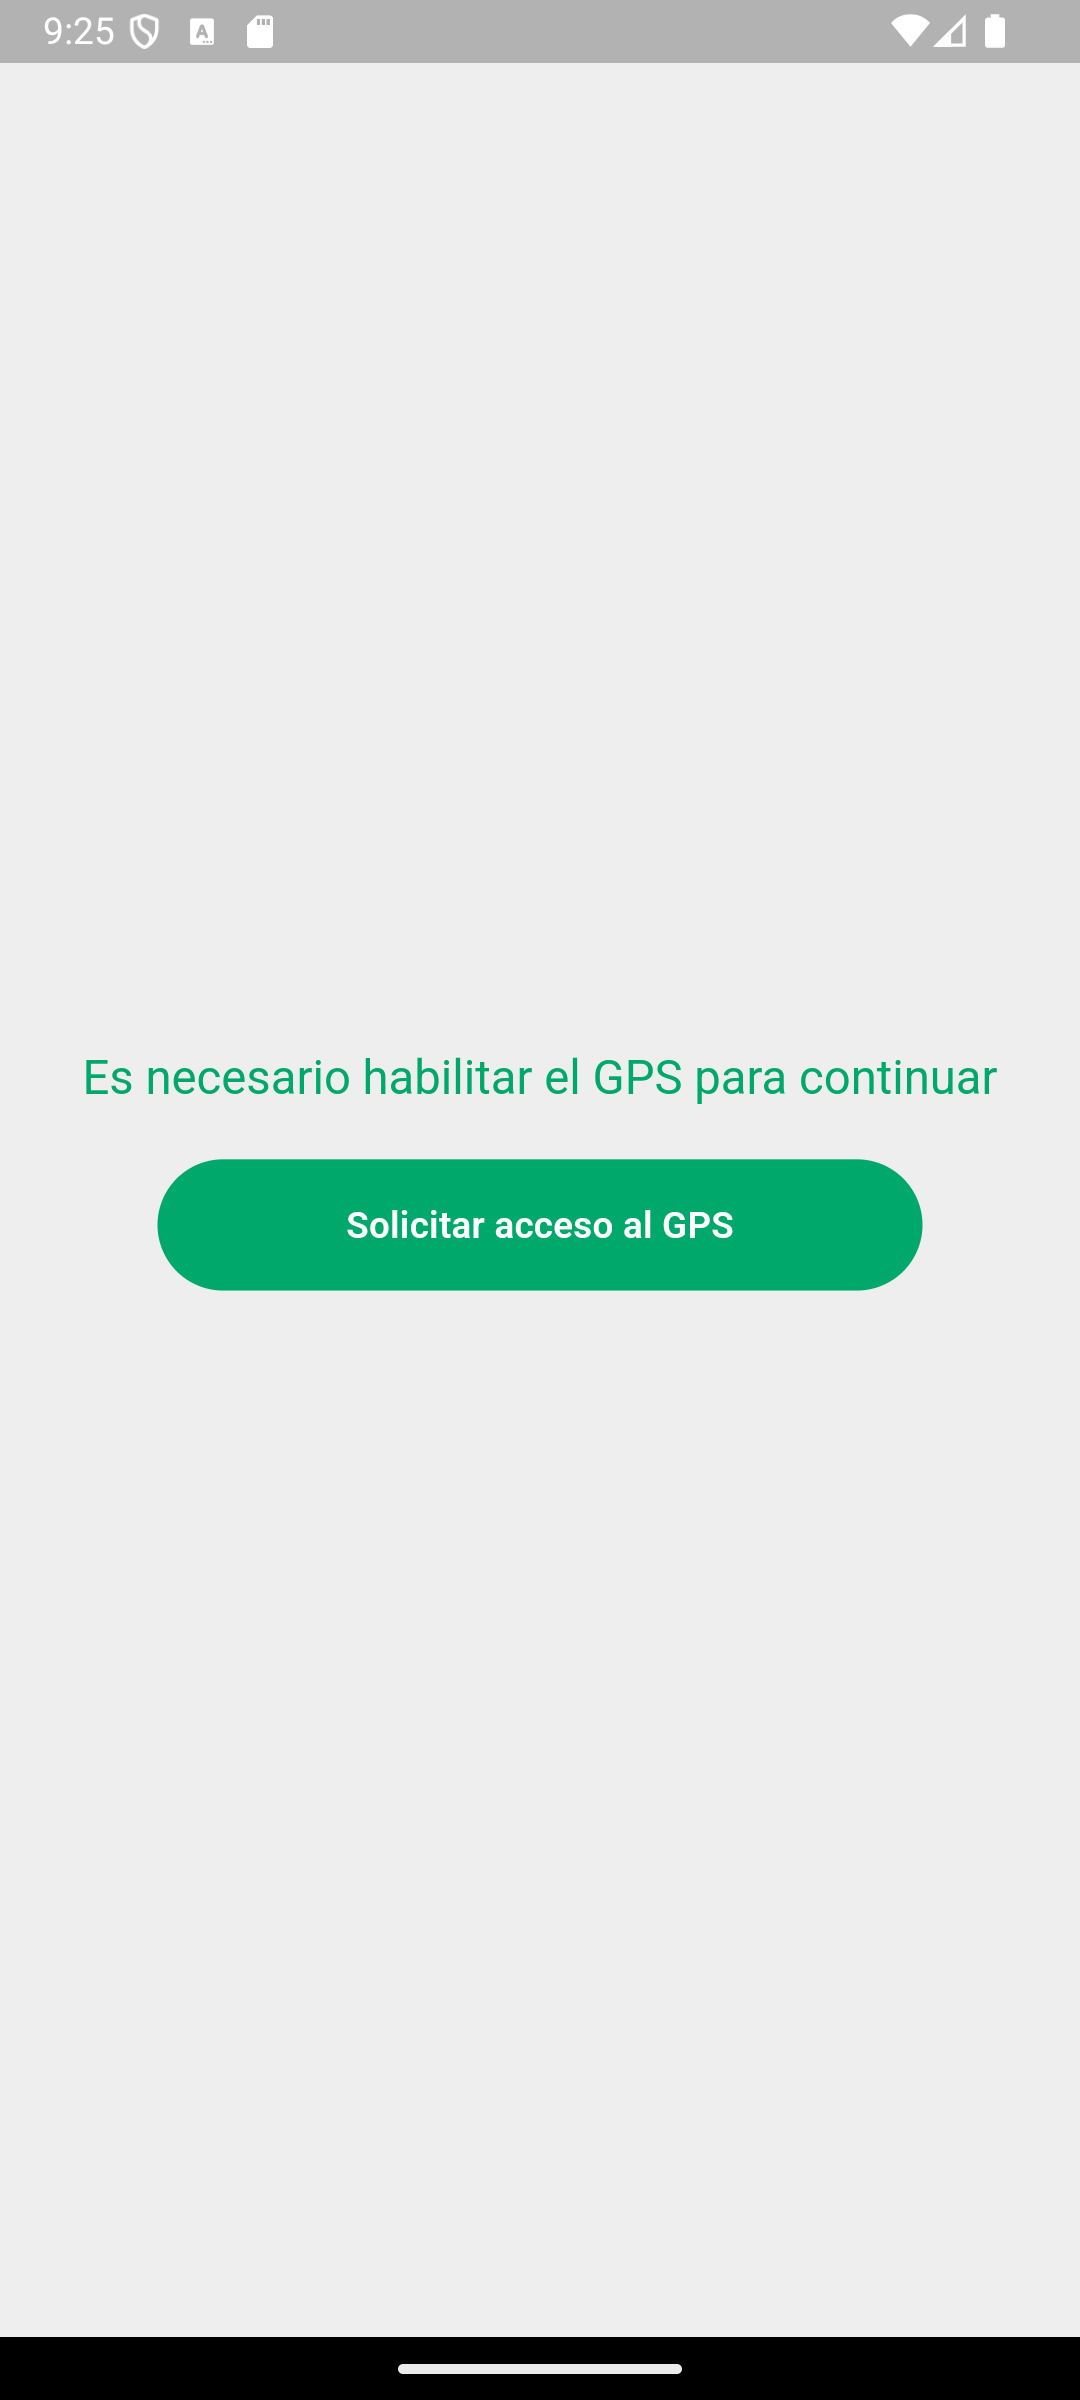
\includegraphics[width=1\linewidth]{E1-habilitar-gps} & 
		\vspace{-10pt}
		
			\begin{flushleft}
				La primera acción que debe realizar el usuario al iniciar la aplicación es habilitar el permiso de uso de GPS. Esto permite que la aplicación acceda a la ubicación del dispositivo para calcular rutas y mostrar información relevante.
				\textbf{Pasos a seguir:}
			\end{flushleft}
			\begin{enumerate}
				\item Al abrir la aplicación por primera vez, aparecerá la pantalla mostrada en la Figura~\ref{fig:habilitarGPS}.
				\item Pulse el botón \textbf{Solicitar acceso al GPS}.
				\item Conceda el permiso solicitado en la ventana emergente.
			\end{enumerate}		
			La aplicación detecta igualmente el uso de GPS deshabilitado y en cualquier momento si se desactiva o se quitan los permisos volvería a esta pantalla.
	\end{tabular}
	\caption{Habilitar el permiso de uso de GPS}
	\label{fig:habilitarGPS}
\end{figure}

\newpage
\subsection{Pantalla de configuración de Eco City Tour}
\begin{figure}[H]
	\centering
		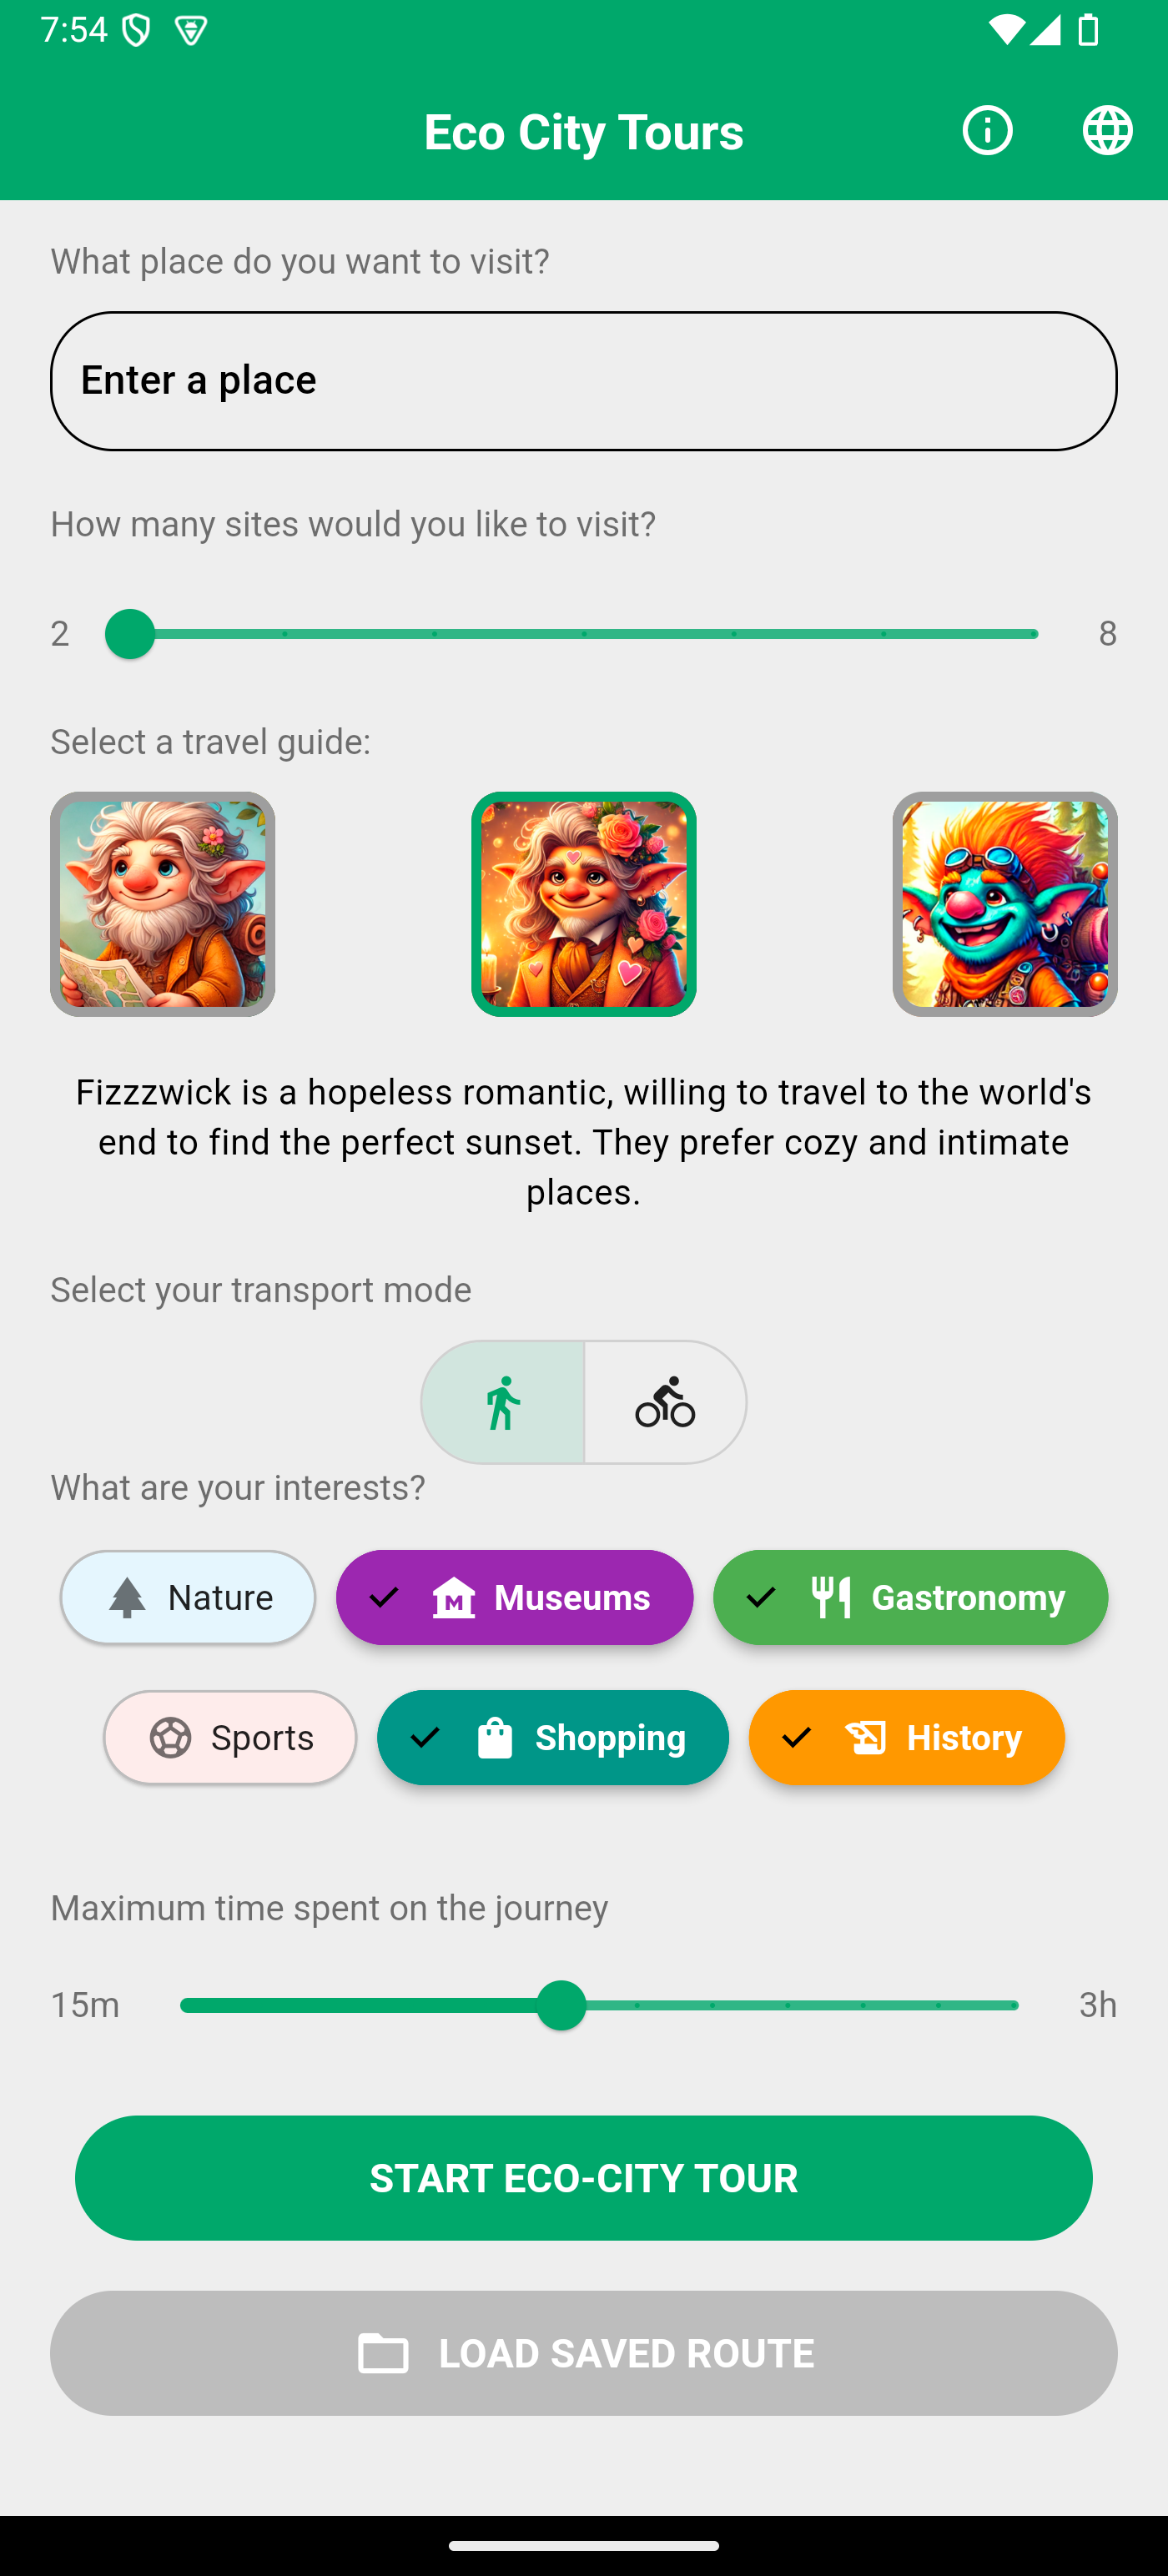
\includegraphics[width=0.4\linewidth]{E2-selection-tour-screen} 	
		\label{fig:selectionTourScreen}
		\caption{Pantalla de configuración de Eco City Tour}
		
	\begin{flushleft}
		Una vez establecidos los permisos veremos la pantalla de configuración del Eco City Tour, donde seleccionaremos nuestras preferencias a la hora de diseñar un tour turístico ecológico por un lugar.
	\end{flushleft}
		\textbf{Pasos a seguir:}
		\begin{enumerate}
			\item En primer lugar introducir la ciudad o sitio que se quiera visitar. 
			\item Se seleccionará cuantos \acrlong{pdi} queremos visitar.
			\item Se seleccionará un asistente si lo deseamos entre las tres opciones disponibles.
			\item Se indicará si queremos hacer la ruta a pie o en bici.
			\item Se indicará nuestras preferencias o gustos a la hora de viajar.
			\item Se indicará un tiempo máximo de tiempo en desplazamientos
			\item Por último se pulsará el botón de \textbf{generar Eco City Tour}
		\end{enumerate}		
	


\end{figure}
\newpage
\subsection{Pantalla de navegación de mapa}
\begin{figure}[H]
	\centering

		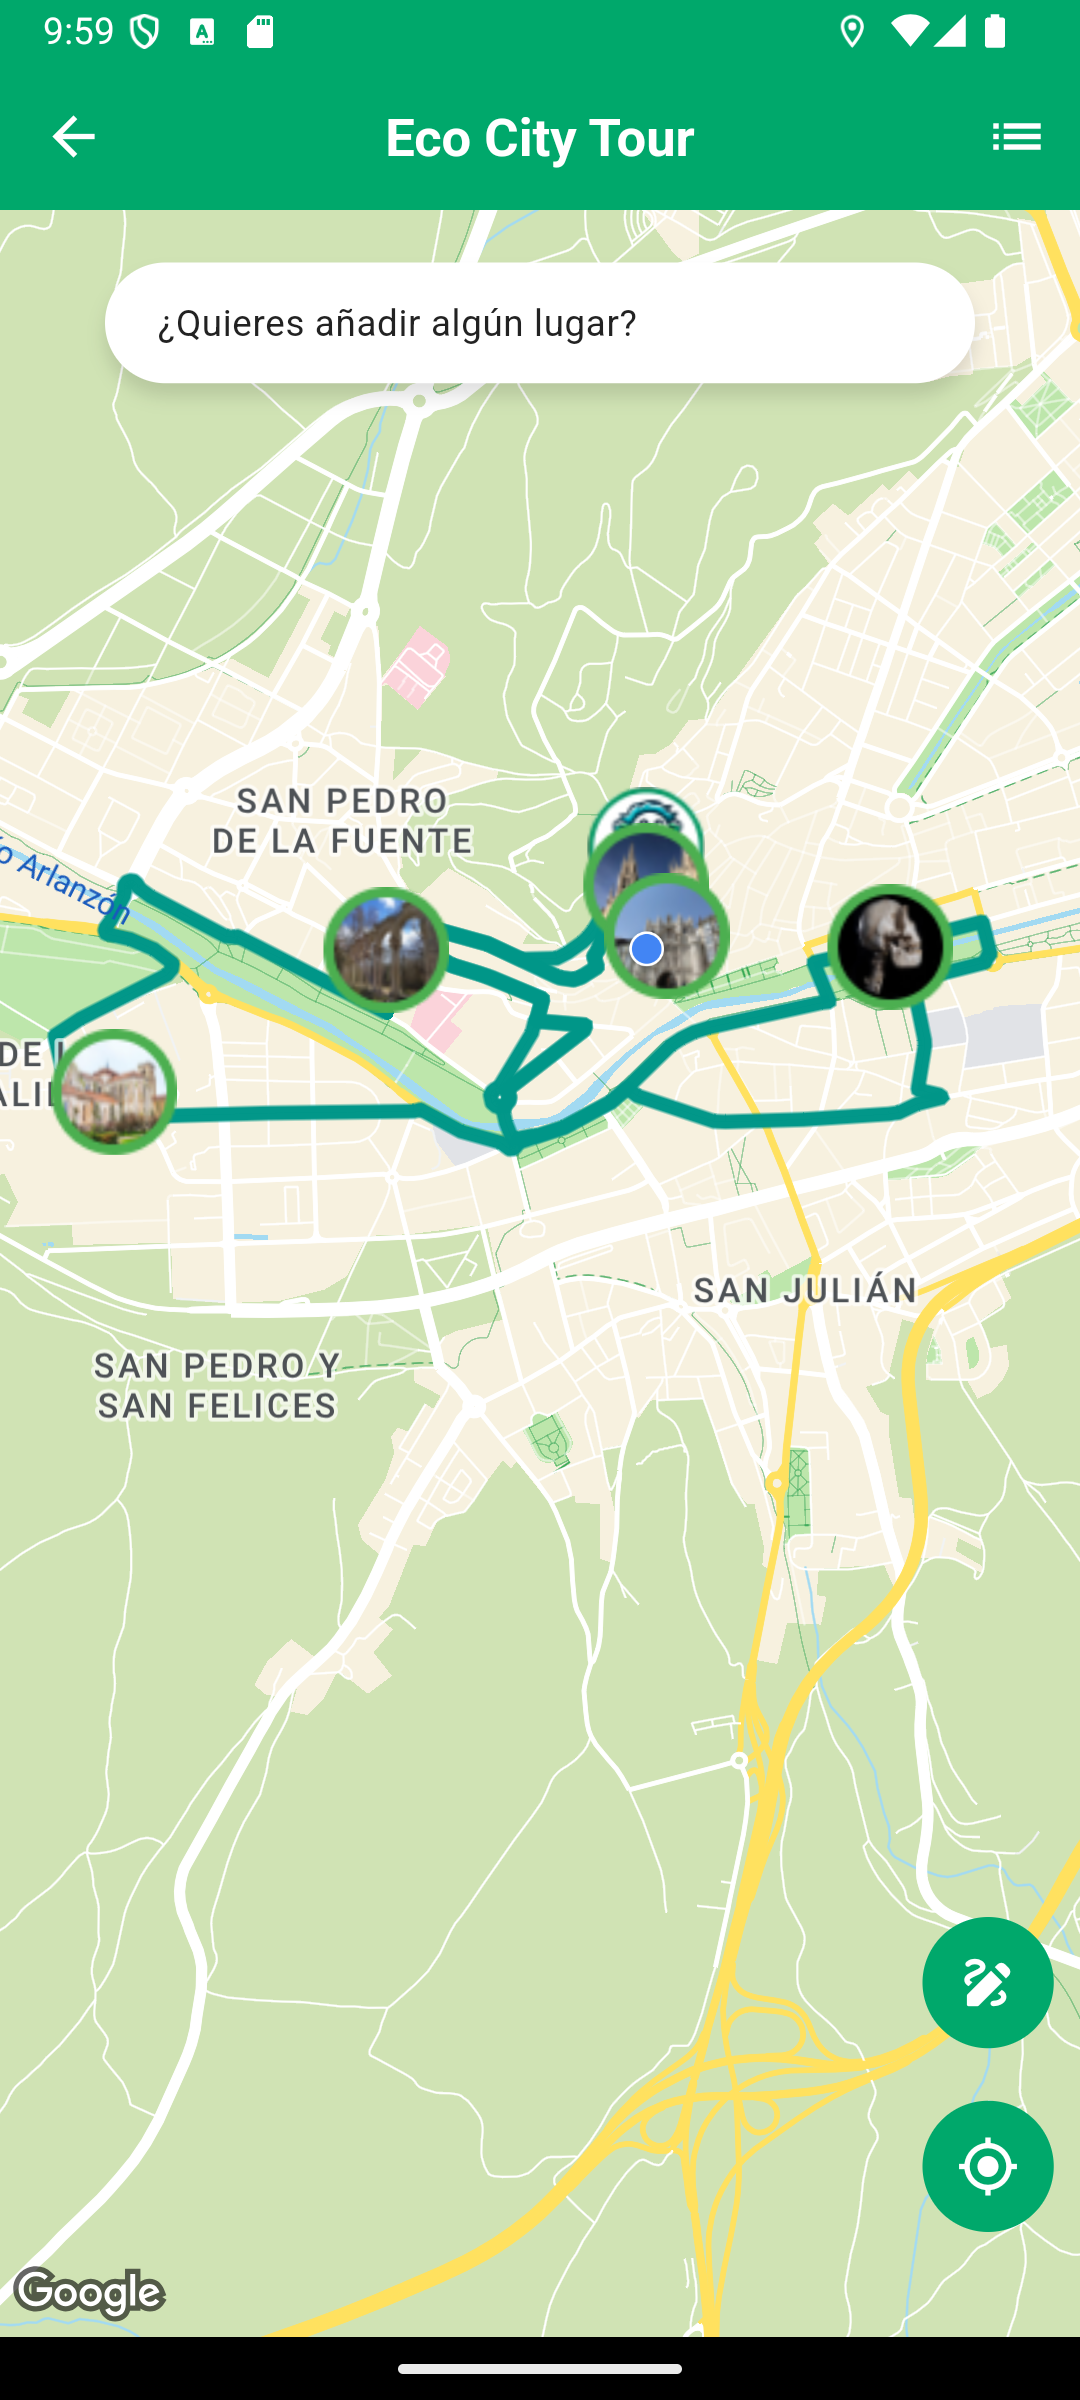
\includegraphics[width=0.4\linewidth]{E3-map-screen}
		\label{fig:navegacionMapa}
		\caption{Pantalla de navegación de mapa}
		
		Una vez cargado el tour podremos navegar por el mapa visualizando los distintos \acrshort{pdi} que la aplicación ha seleccionado para visitar, así como una ruta optimizada que une los puntos.
		
		\textbf{Desde aquí hay varias opciones:}
		\begin{itemize}
			\item Eliminar aquellos lugares que no queramos visitar.
			\item Añadir lugares a la ruta. Fig.~\ref{fig:busquedaPDI}
			\item Guardar el Eco City Tour. Fig.~\ref{fig:saveECT}
			\item Unir la posición GPS del usuario a la ruta. Fig.~\ref{fig:joinECT}
			\item Visualizar el seguimiento GPS del usuario. Fig.~\ref{fig:followingUser}
		\end{itemize}		
	
\end{figure}


\subsection{Buscar y añadir un \acrlong{pdi} al Eco City Tour}
\begin{figure}[H]
	\centering
	\begin{tabular}{m{0.4\textwidth} m{0.55\textwidth}}
		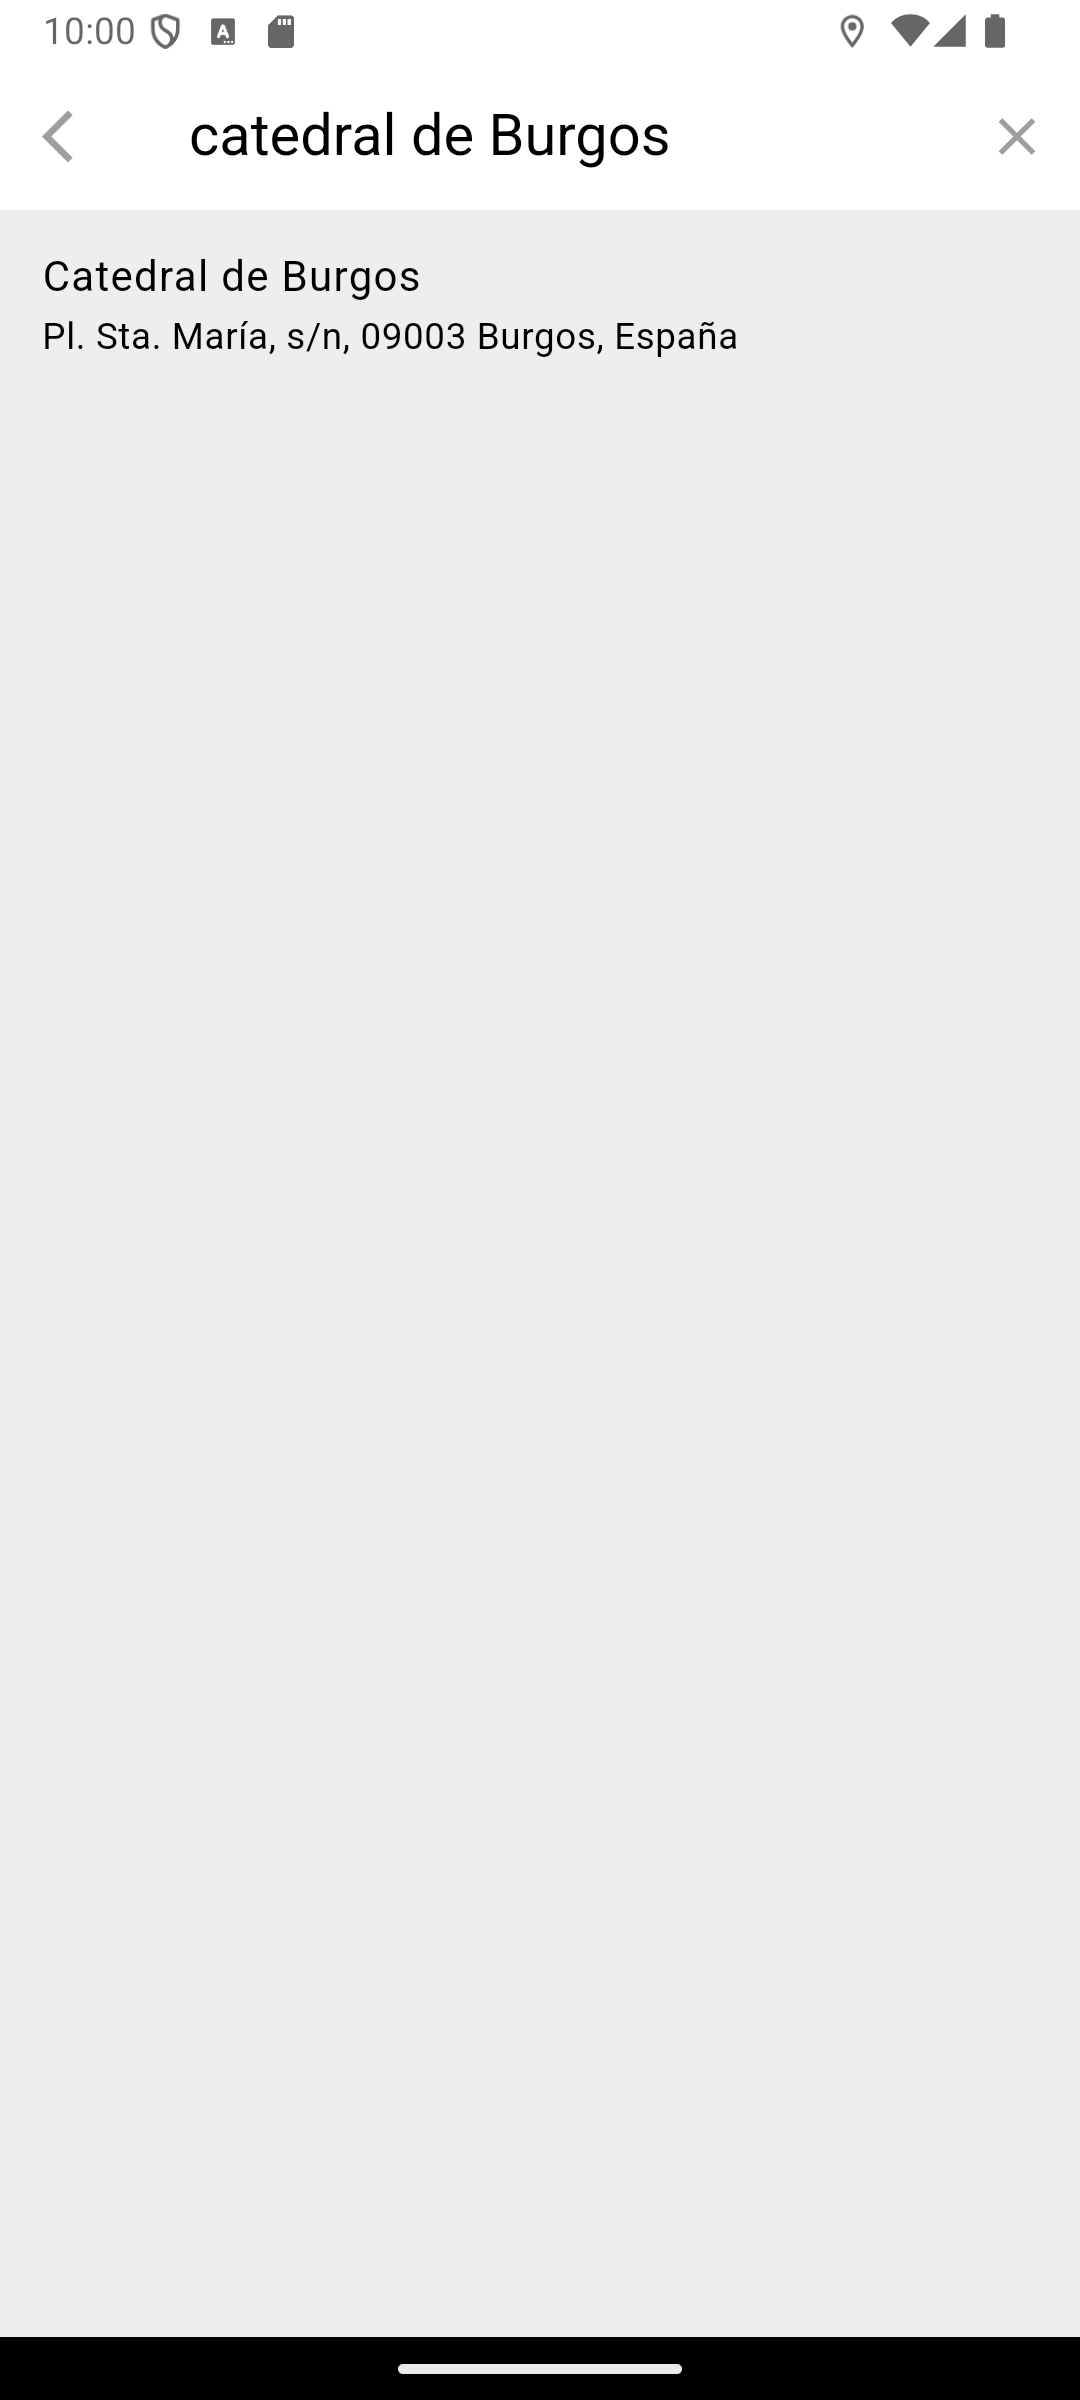
\includegraphics[width=0.6\linewidth]{E4-search-bar} & 
		\vspace{-10pt}
		Si el usuario conoce un lugar o desea añadir algún tipo de comercio (hospital, parque, supermercado) a la ruta solo tiene que seguir los pasos desde la Fig.~\ref{fig:navegacionMapa} 
		
		\textbf{Pasos a seguir:}
		\begin{enumerate}
			\item Introduce el nombre del lugar/lugares que quieras buscar en la barra de búsqueda. Por ejemplo en la Fig.~\ref{fig:busquedaPDI} se busca "Catedral de Burgos", mostrando un solo resultado 
			\item El usuario pulsará sobre el resultado que desea añadir.
			\item El sistema añade el lugar a la ruta y recalcula el camino más corto.
		\end{enumerate}		
	\end{tabular}
	\caption{Búsqueda de \acrshort{pdi}}
	\label{fig:busquedaPDI}
\end{figure}


\subsection{Conocer detalle de \acrshort{pdi}}
\begin{figure}[H]
	\centering
	\begin{tabular}{m{0.4\textwidth} m{0.55\textwidth}}
		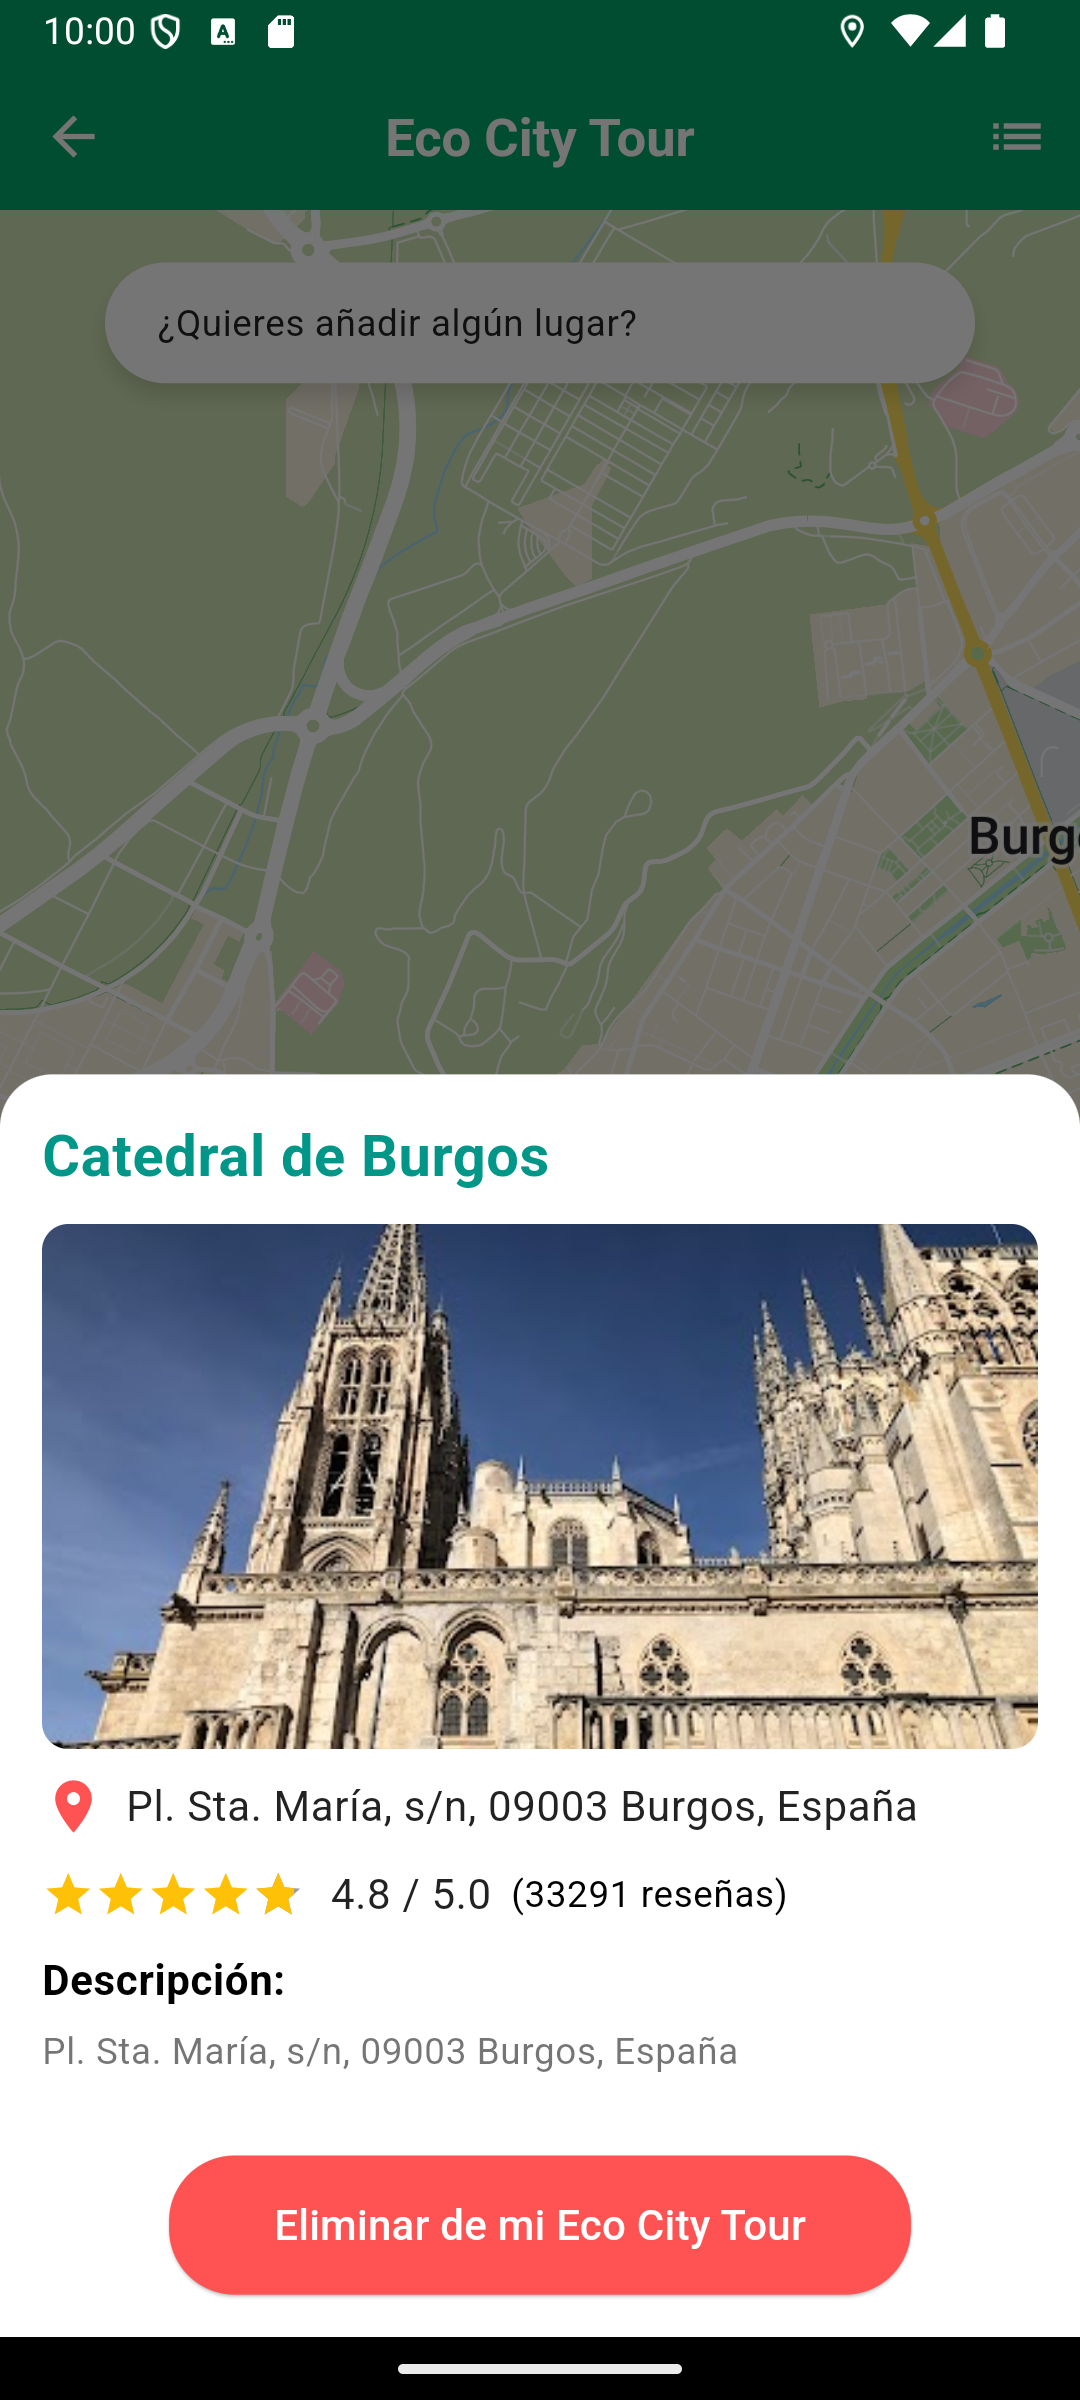
\includegraphics[width=0.6\linewidth]{E5-PDI-detalle} & 
		\vspace{-10pt}
		Uno de los elementos básicos de la navegación en el mapa que podemos ver en la Fig.~\ref{fig:navegacionMapa} es la de buscar información de un \acrlong{pdi} al seleccionar un elemento se nos muestra una imagen, una descripción, una valoración entre las obtenidas en Google y la opción de eliminar la visita del tour si no es de nuestro agrado. 
	\end{tabular}
	\caption{Detalle de \acrshort{pdi}}
	\label{fig:detallePDI}
\end{figure}

\subsection{Resumen de Eco City Tour creado}
\begin{figure}[H]
	\centering
	\begin{tabular}{m{0.4\textwidth} m{0.55\textwidth}}
		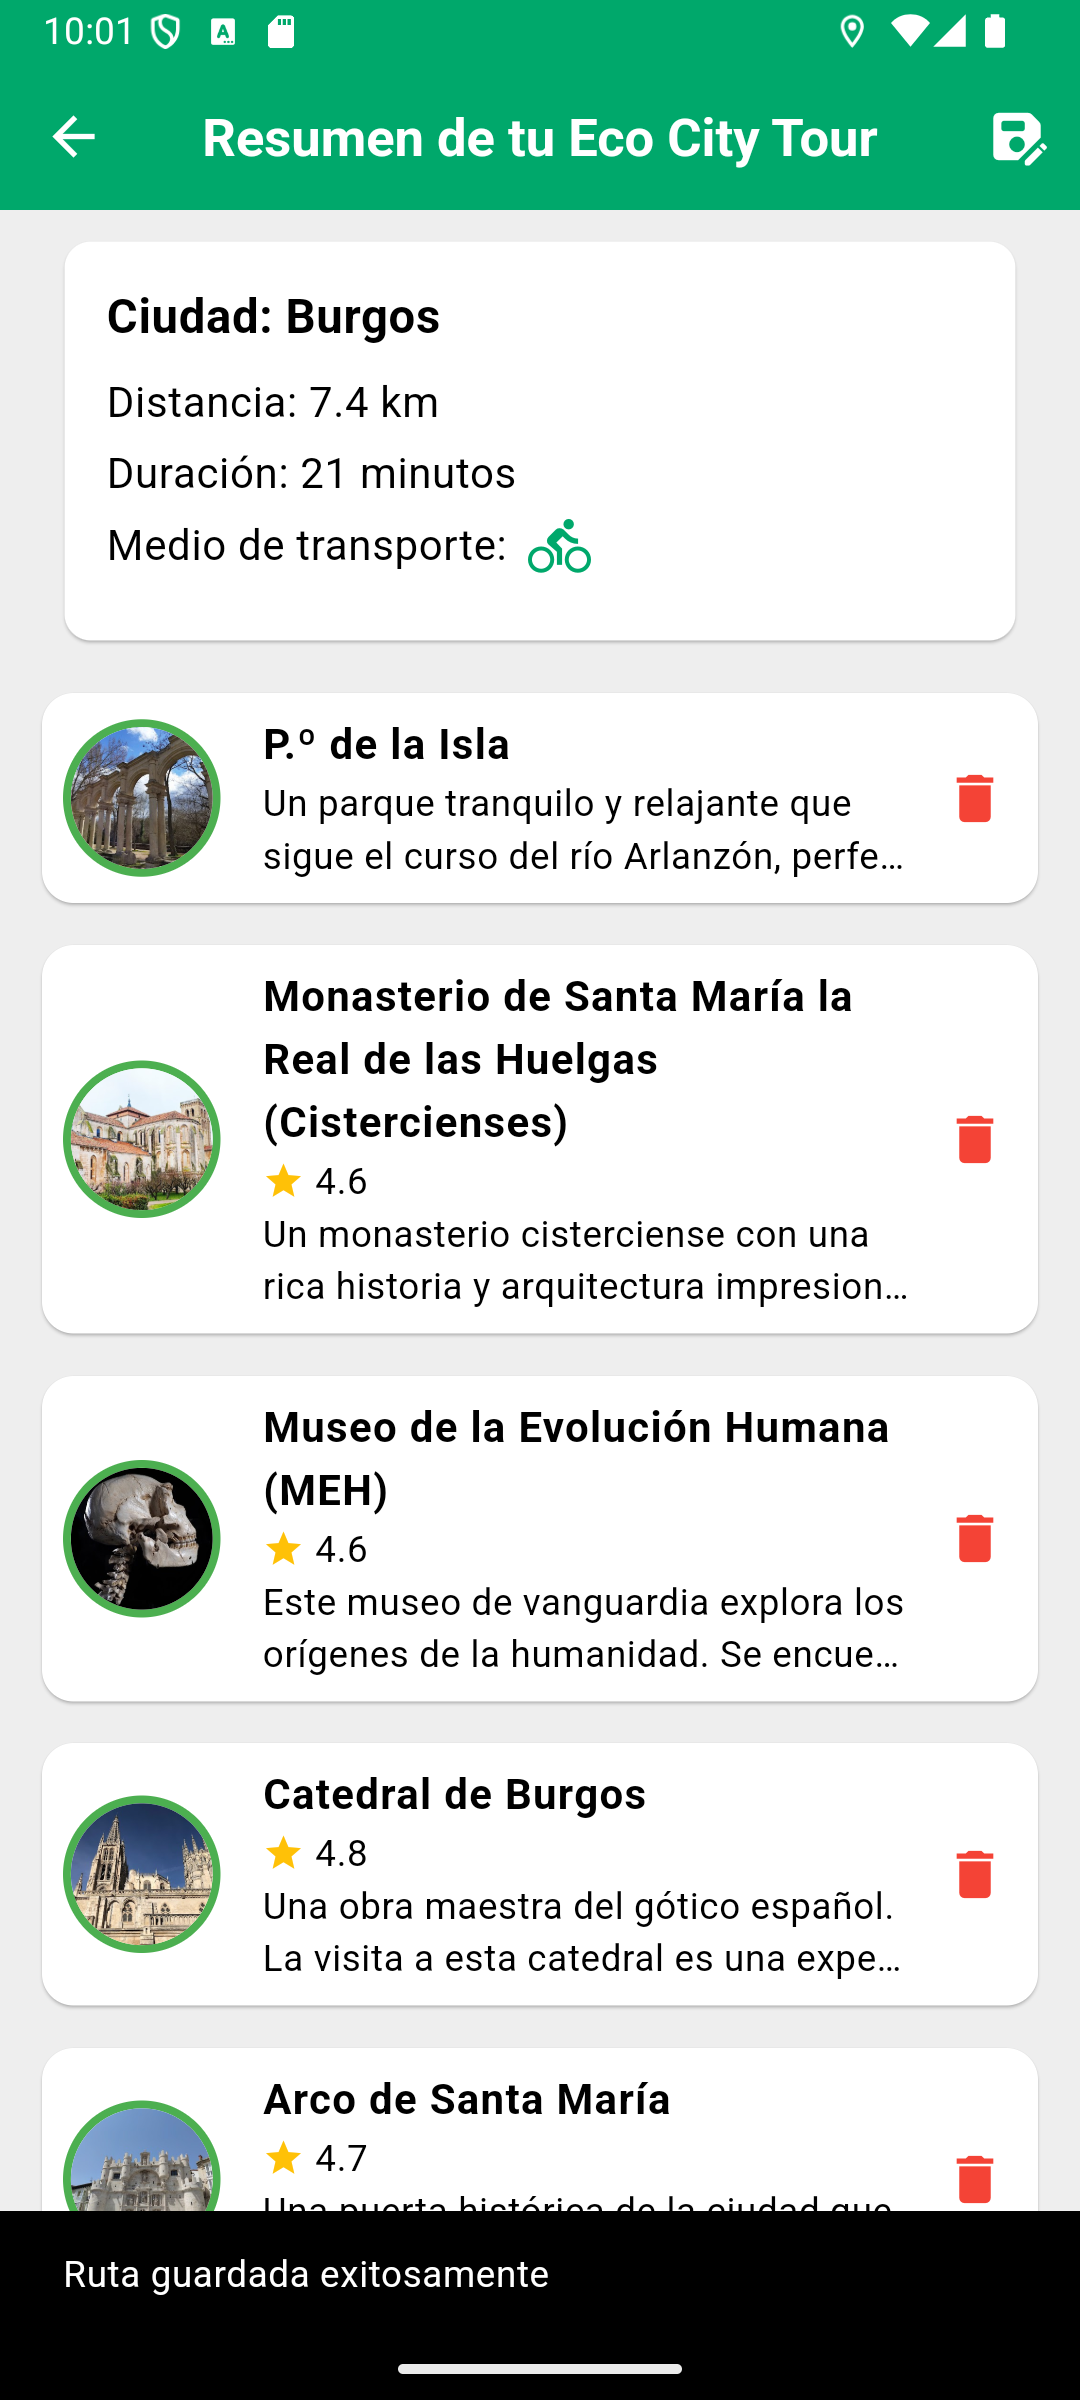
\includegraphics[width=0.6\linewidth]{E6-summary-screen} & 
		\vspace{-10pt}
		Desde el mapa podemos acceder a esta ventana que nos mostrará en su parte superior un resumen de las características del tour y en la parte inferior cada uno de los \acrlong{pdi} que forman el Eco City Tour.
		
		\textbf{Opciones:}
		\begin{enumerate}
			\item Podemos ampliar la información de la descripción.
			\item Eliminar del Eco City Tour un \acrshort{pdi}
			\item Guardar el Eco City Tour actual (Fig.~\ref{fig:saveECT}) o volver al mapa (Fig.~\ref{fig:navegacionMapa})
		\end{enumerate}		
	\end{tabular}
	\caption{Pantalla de resumen del Eco City Tour}
	\label{fig:resumenECT}
\end{figure}

\subsection{Guardar Eco City Tour}
\begin{figure}[H]
	\centering
	\begin{tabular}{m{0.4\textwidth} m{0.55\textwidth}}
		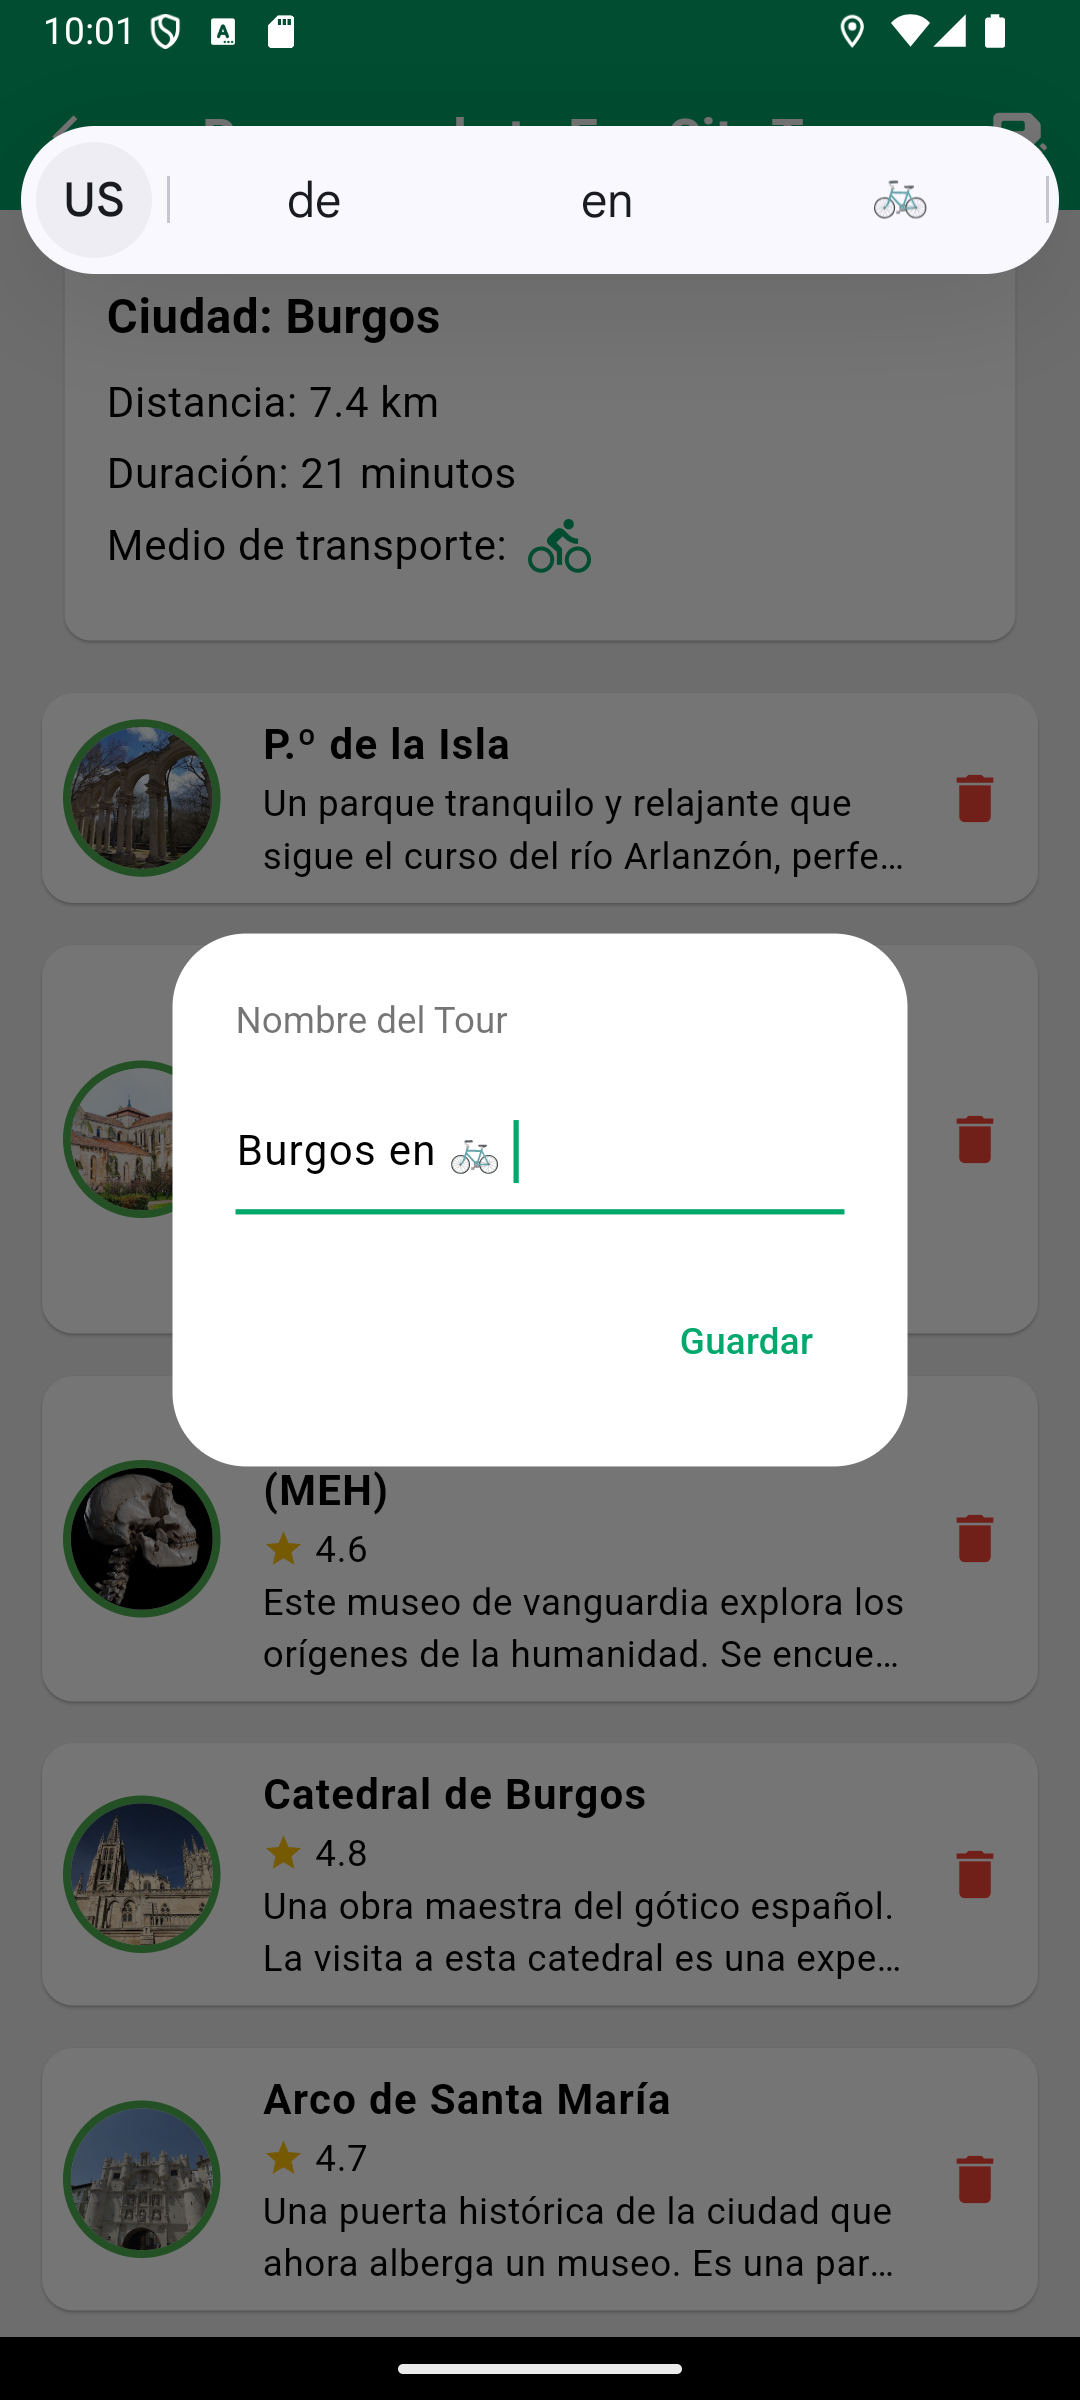
\includegraphics[width=0.6\linewidth]{E7-save-tour} & 
		\vspace{-10pt}
		Si queremos guardar la ruta para verla en otra ocasión el usuario puede guardar la información.
		\textbf{Pasos a seguir:}
		\begin{enumerate}
			\item Desde la pantalla de resumen del Eco City Tour, pulsar el botón de guardado de ruta.
			\item Elegimos un nombre.
			\item Un mensaje en la parte inferior nos informará que el Eco City Tour ha sido guardado con éxito.
		\end{enumerate}		
	\end{tabular}
	\caption{Pantalla de guardado del Eco City Tour}
	\label{fig:saveECT}
\end{figure}

\subsection{Cargar Eco City Tour}
\begin{figure}[H]
	\centering
	\begin{tabular}{m{0.4\textwidth} m{0.55\textwidth}}
		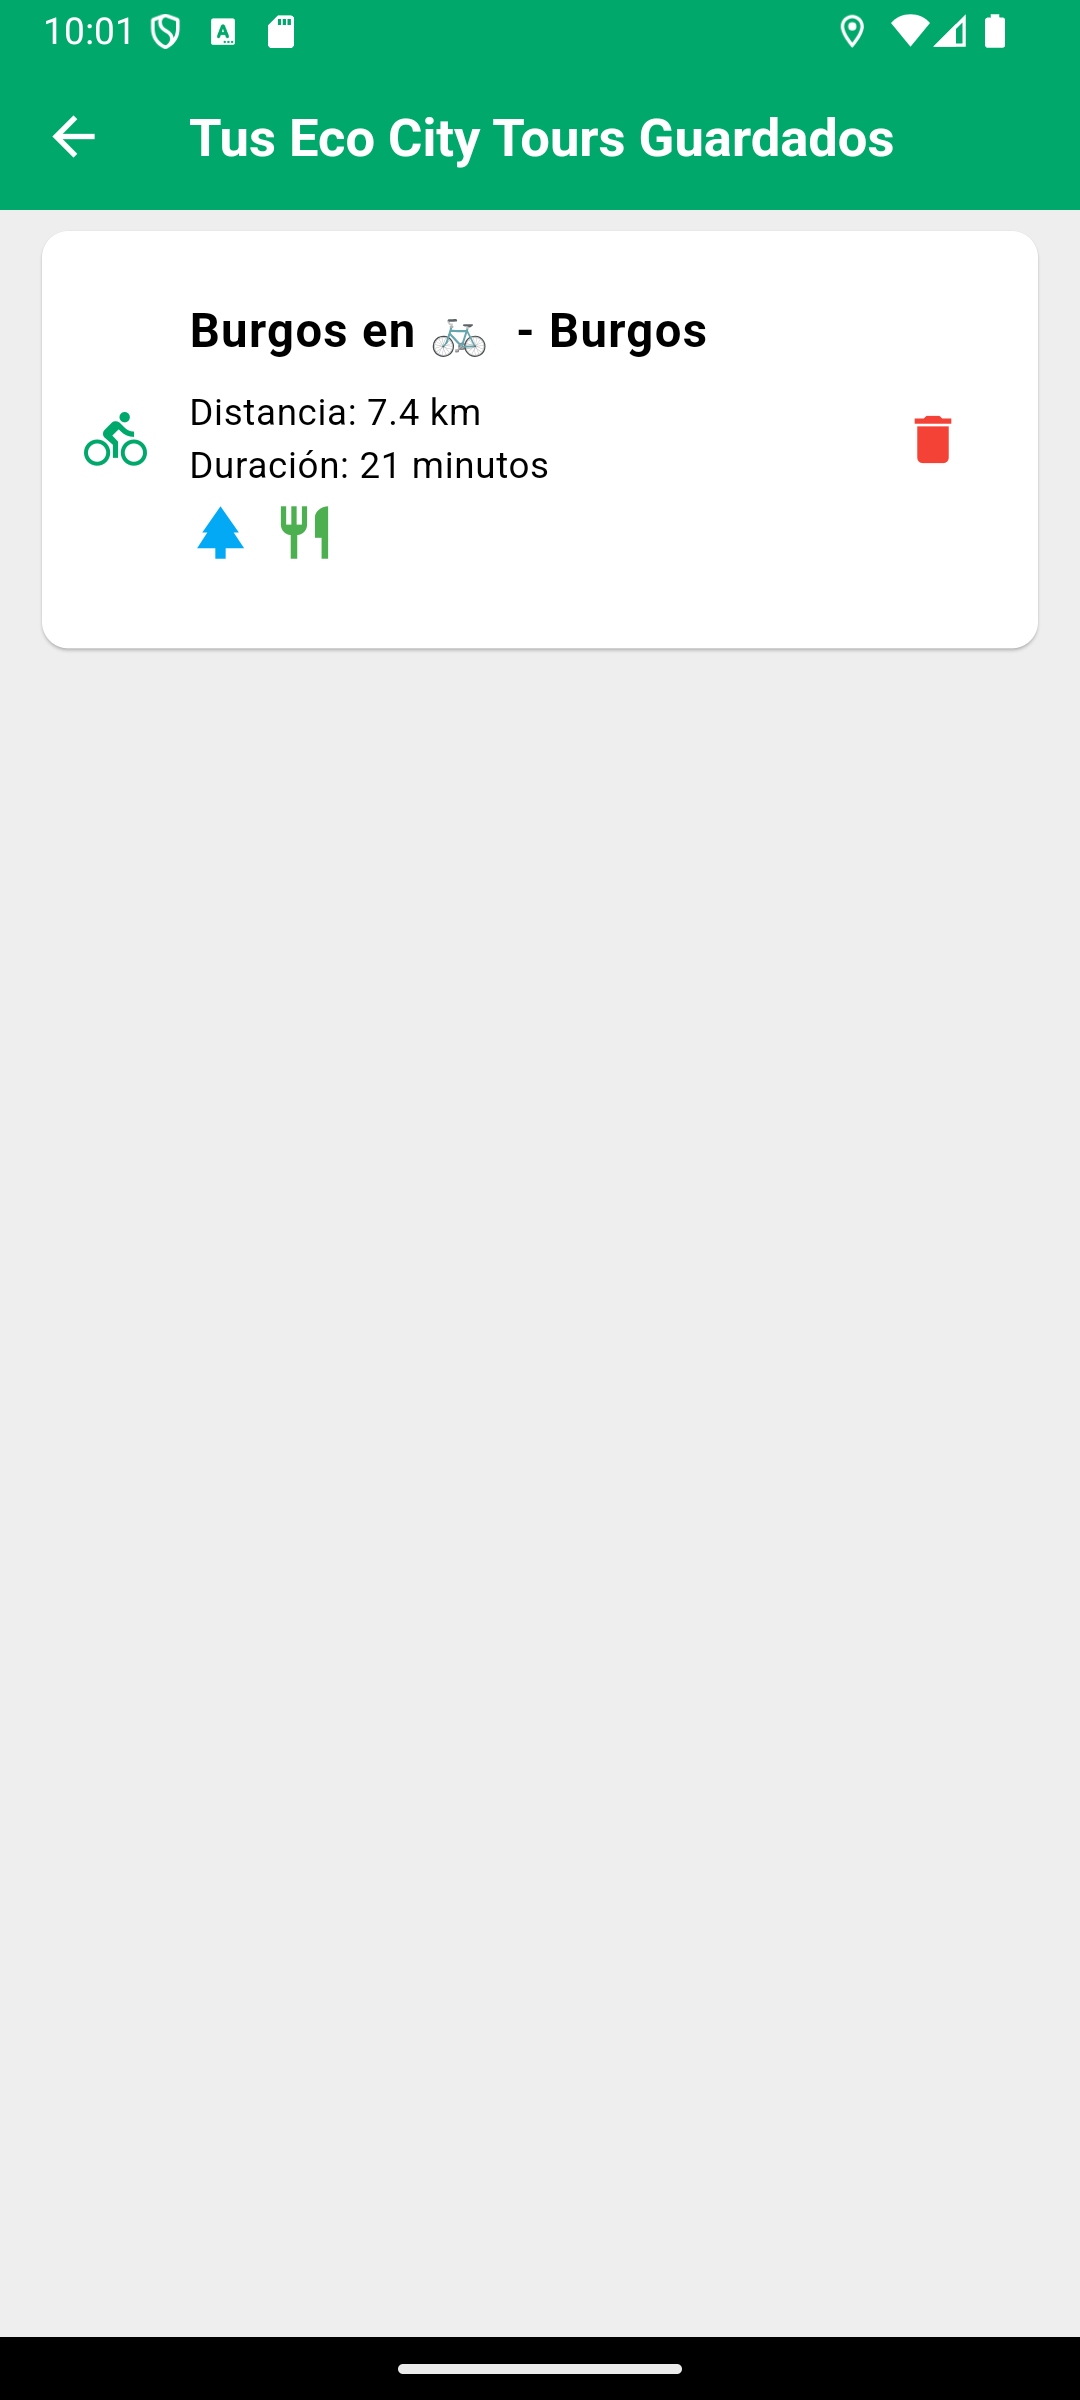
\includegraphics[width=0.6\linewidth]{E8-load-tour} & 
		\vspace{-10pt}
		Desde la pantalla de configuración (Figura~\ref{fig:selectionTourScreen}) podemos ver todos nuestras rutas personales guardadas.
		Simplemente seleccionaremos sobre el Eco City Tour que queramos cargar sobre el mapa y la pantalla de navegación del mapa  (Fig.~\ref{fig:navegacionMapa}) se mostrará en el mapa con el Eco City Tour guardado, mostrando la información relevante y todos los \acrlong{pdi}.	
	\end{tabular}
	\caption{Pantalla de carga del Eco City Tour}
	\label{fig:loadECT}
\end{figure}

\subsection{Unirse al Eco City Tour}
\begin{figure}[H]
	\centering
	\begin{tabular}{m{0.4\textwidth} m{0.55\textwidth}}
		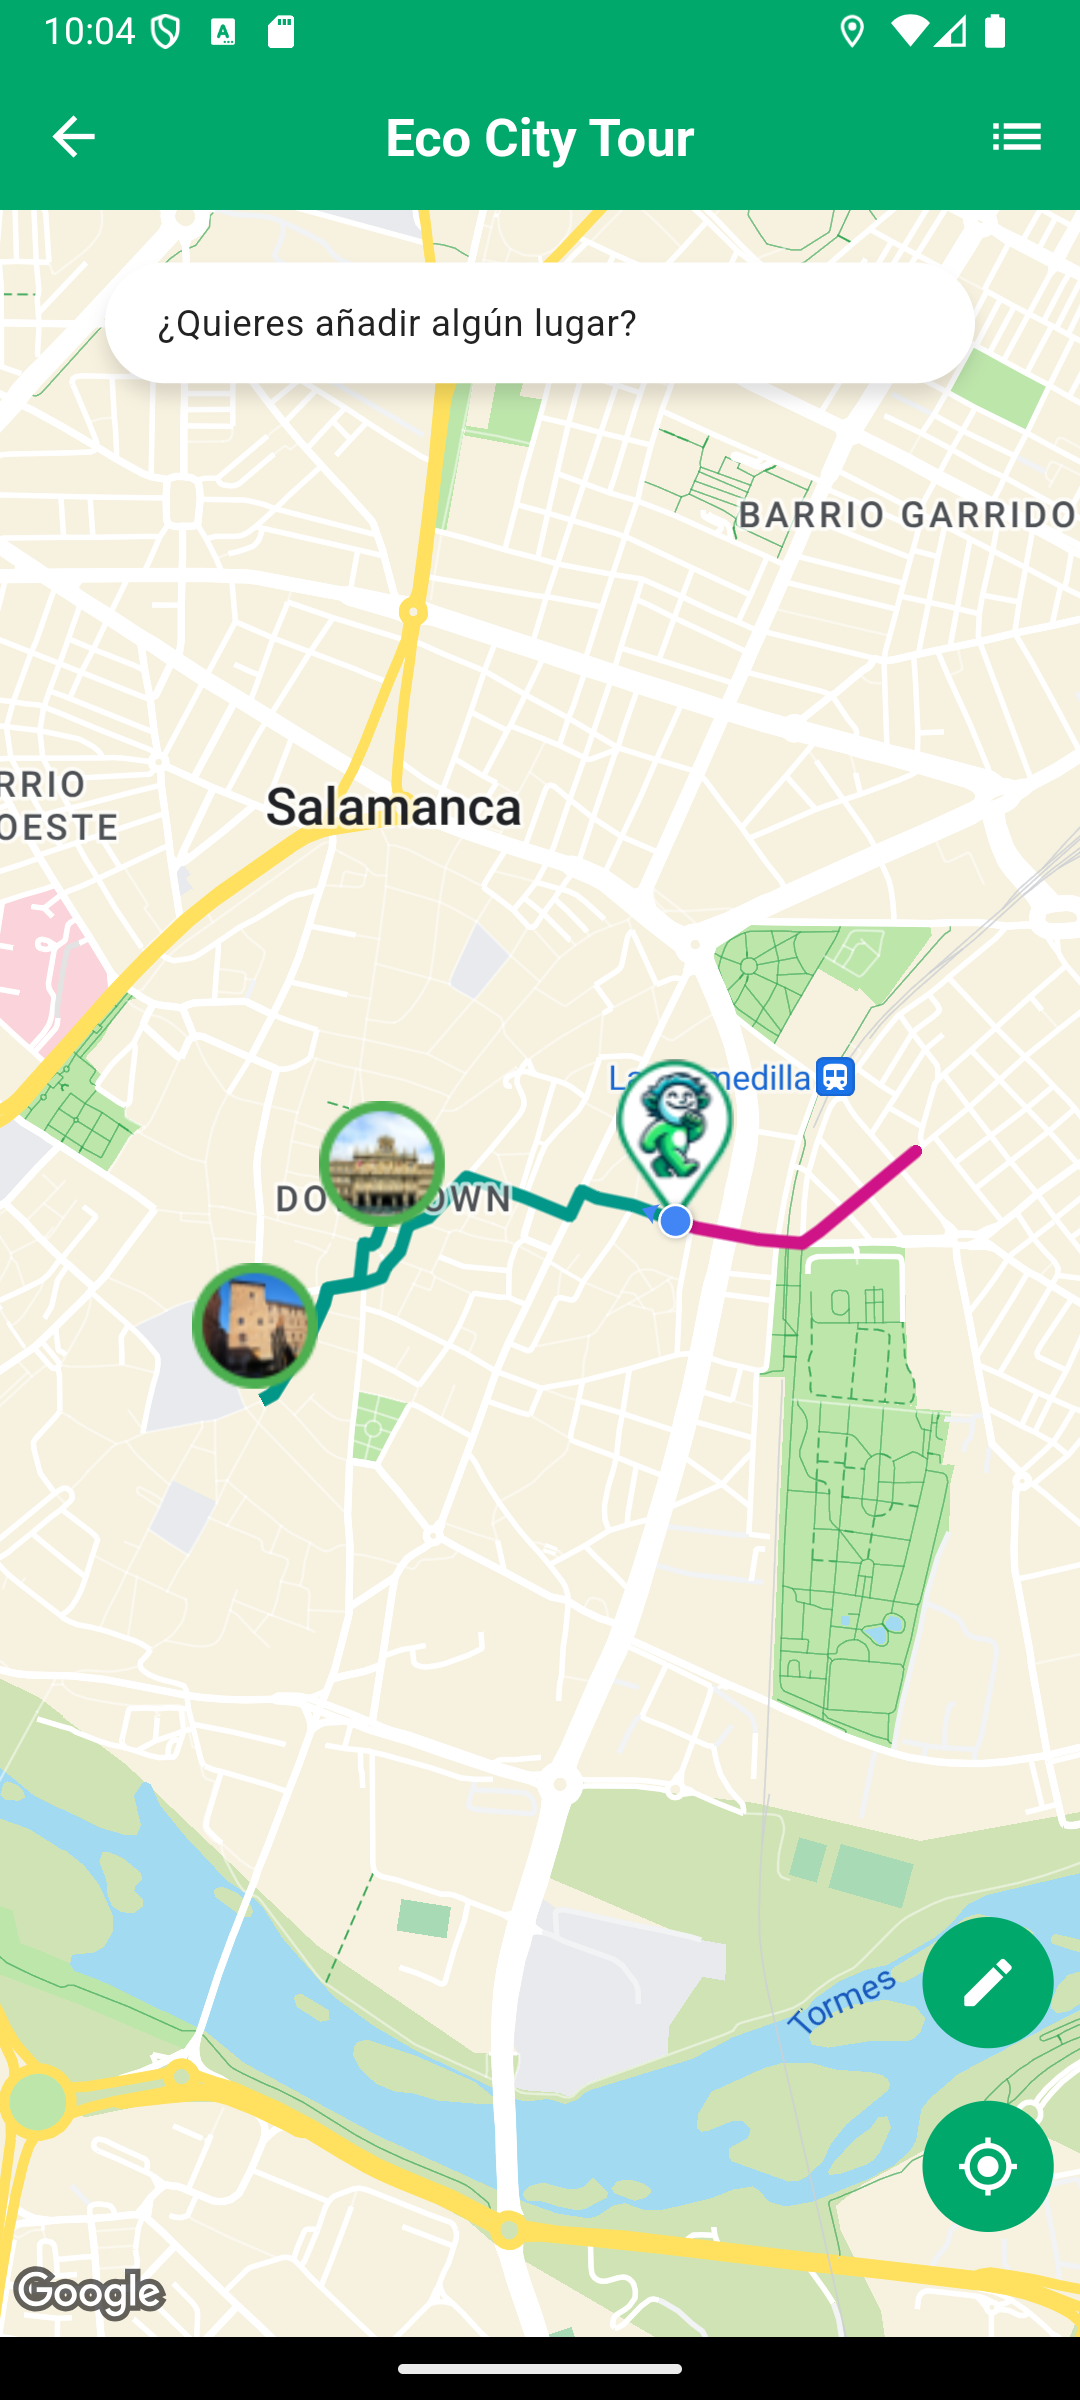
\includegraphics[width=0.6\linewidth]{E10-join-tour} & 
		\vspace{-10pt}
		Precisamente si el usuario está en un sitio clave que no quiere perder o simplemente quiere que la ubicación forme parte del Eco City Tour puede pulsar el botón inferior de la pantalla del mapa (Fig.~\ref{fig:navegacionMapa}) y se añadirá un nuevo \acrshort{pdi} con la ubicación del usuario y se recalculará de nuevo la ruta más corta entre los puntos que estaban creados y la posición del usuario.
		
		Como si de un \acrlong{pdi} corriente se tratase se puede eliminar en cualquier momento.
	\end{tabular}
	\caption{Unirse al Eco City Tour}
	\label{fig:joinECT}
\end{figure}

\subsection{Seguimiento en vivo de la posición del usuario}
\begin{figure}[H]
	\centering
	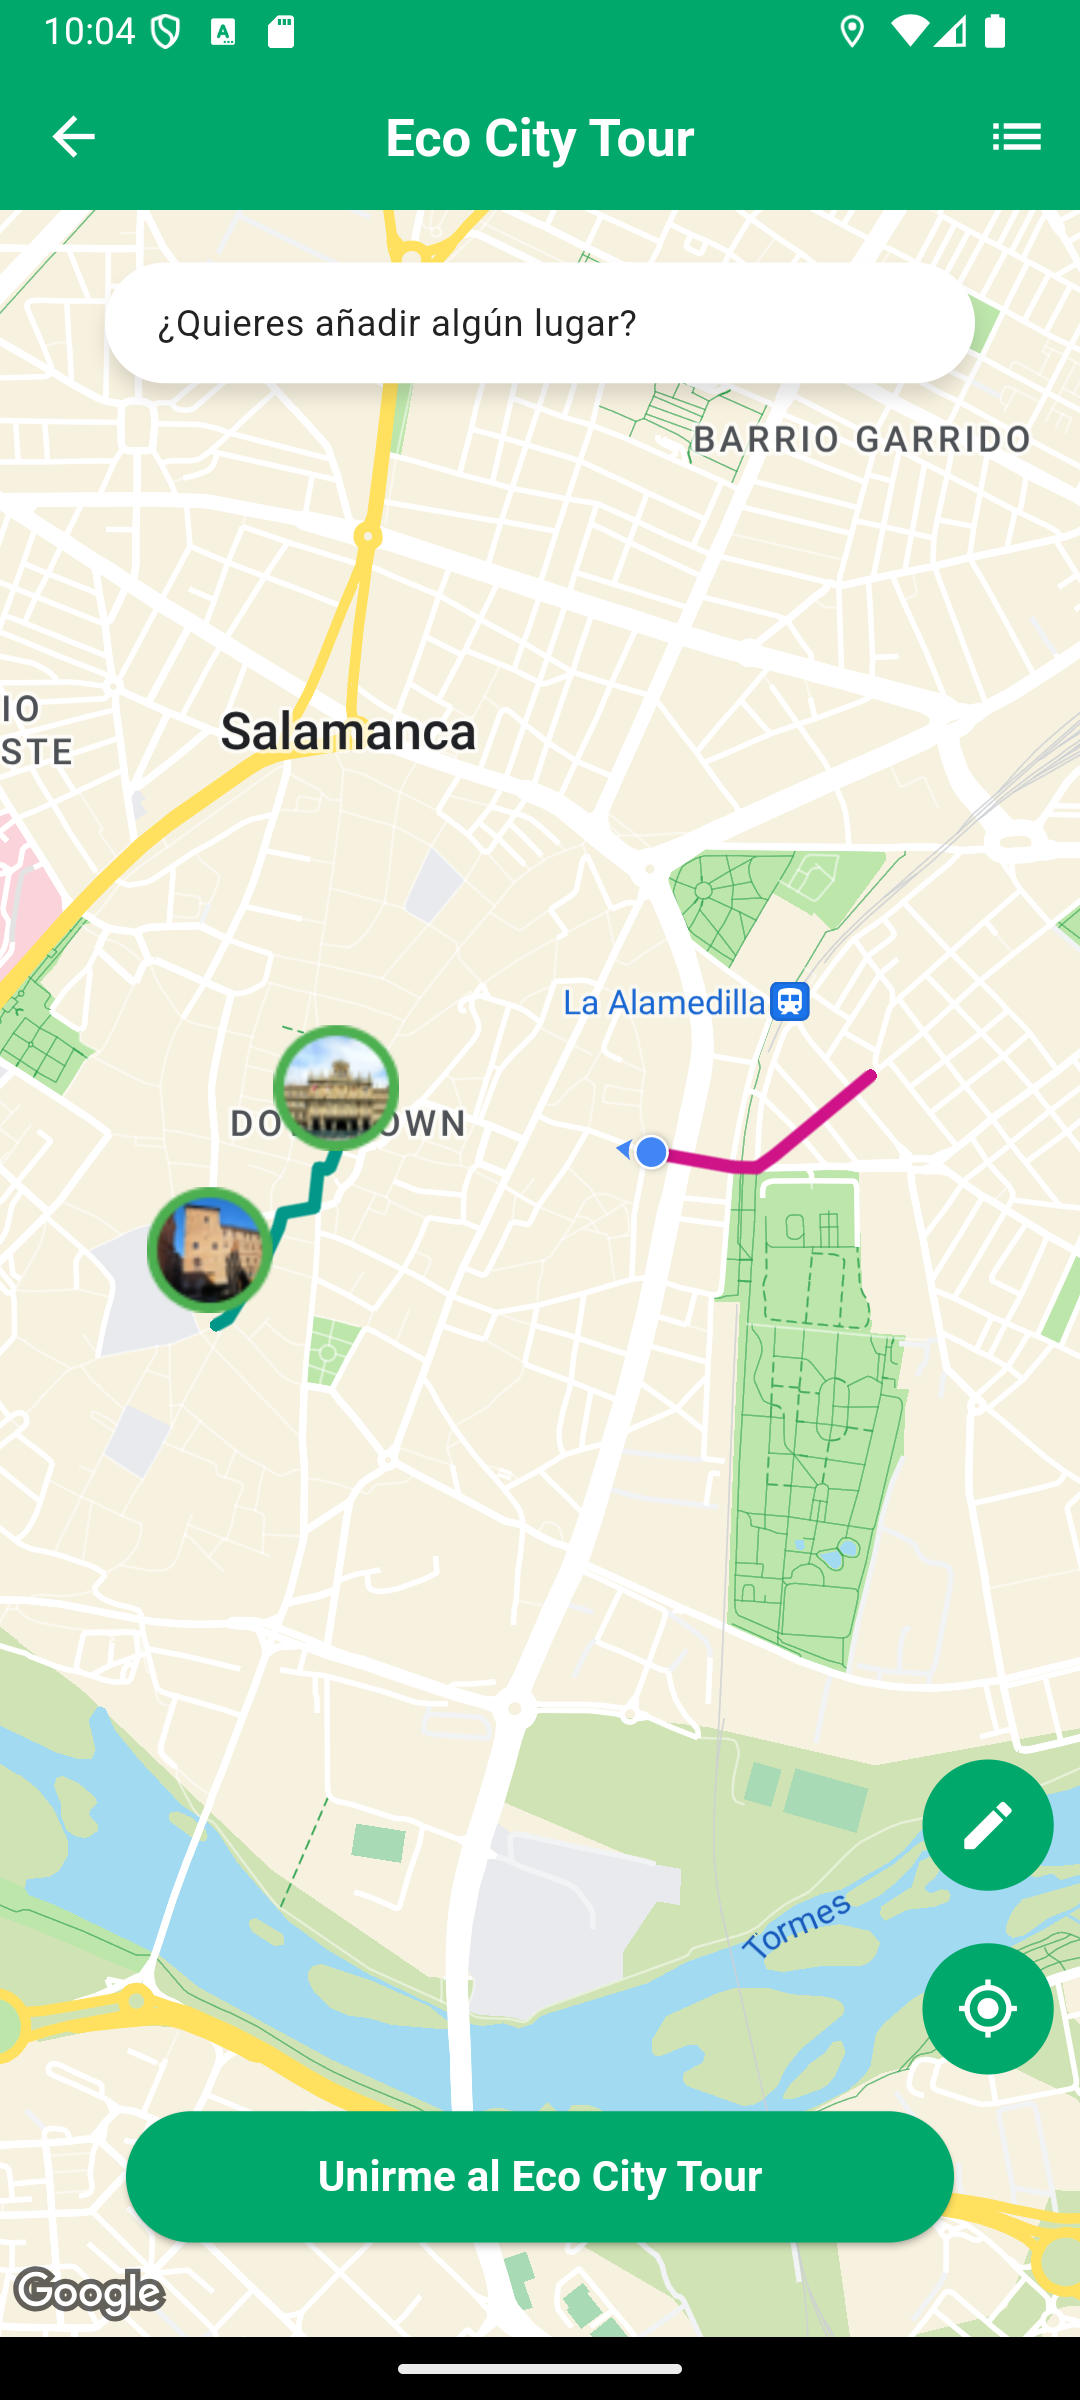
\includegraphics[width=0.35\linewidth]{E9-following-user} 
	\caption{Seguimiento en vivo de la posición del usuario}
	\label{fig:followingUser}
	\vspace{-10pt}
\end{figure}

Otras opciones que se pueden llevar a cabo desde la pantalla de navegación del mapa (Fig.~\ref{fig:navegacionMapa}) las llevamos a cabo con los botones flotantes inferiores, tenemos los dos siguientes:
		
\begin{enumerate}
	\item Permite que se muestre sobre pantalla un seguimiento del usuario, el camino que ha seguido se mostrará en el mapa y podrá comprobar su recorrido en todo momento. Para desactivar la línea solo tenemos que pulsar de nuevo el mismo botón.
	\item El segundo botón centrará la pantalla del mapa sobre la ubicación actual del dispositivo y permanecerá así hasta que se mueva de nuevo la pantalla.
\end{enumerate}		

Estas opciones amplían la funcionalidad de un turista, permitiendo controlar en todo momento su recorrido.






